\chapter{Analisi}
In qeusto capitolo analizzero il ragiornamento che ci ha portato all'implementazione dei nostri esperimenti.

In particolar modo ci concentraremo sulle decisioni che sono state prese riguardo al representation language. Una volta che abbiamo deciso come volgiamo che il sistema ci spieghi il fatto su cui facciamo inferenza, cioè definito lo spazio di ricerca, diventa semplice definire la background knowloedge e le etihette degli esempi di training.

%%%%%%%%%%%%%%%%%%%%%%%%%%%%%%%%%%%%%%%%%
\section{Gestione delle tracce}
Un punto cruciale è stato definire come il sistema deve gestire stessi task in tracce diverse. Deve infatti essere consapevole che due task in tracce diverse che hanno lo stessi ID rappresentano la stessa implementazione con le stesse caratteristiche, ma non deve produrre una regola usando informazioni proveninti da tracce diverse.

Prendiamo come esempio la Figura~\ref{fig:trace_management}; questa è portata solo come esempio e ha poco senso in uno scenario reale, visto che le due tracce sono identiche. Quello che volgiamo è che il sistema non unisca le informazioni relative a quello che succede al \textit{Task1} nella prima traccia con quello che succede allo stesso task nella seconda traccia. È però importante che sappia che il \textit{Task1} è sempre lo stesso in entrambe le tracce, anche se non conosce le carattersiche esplicite che il modello del sistema potrebbe fornirci.
\begin{wrapfigure}{L}{.4\textwidth}
    \centering
    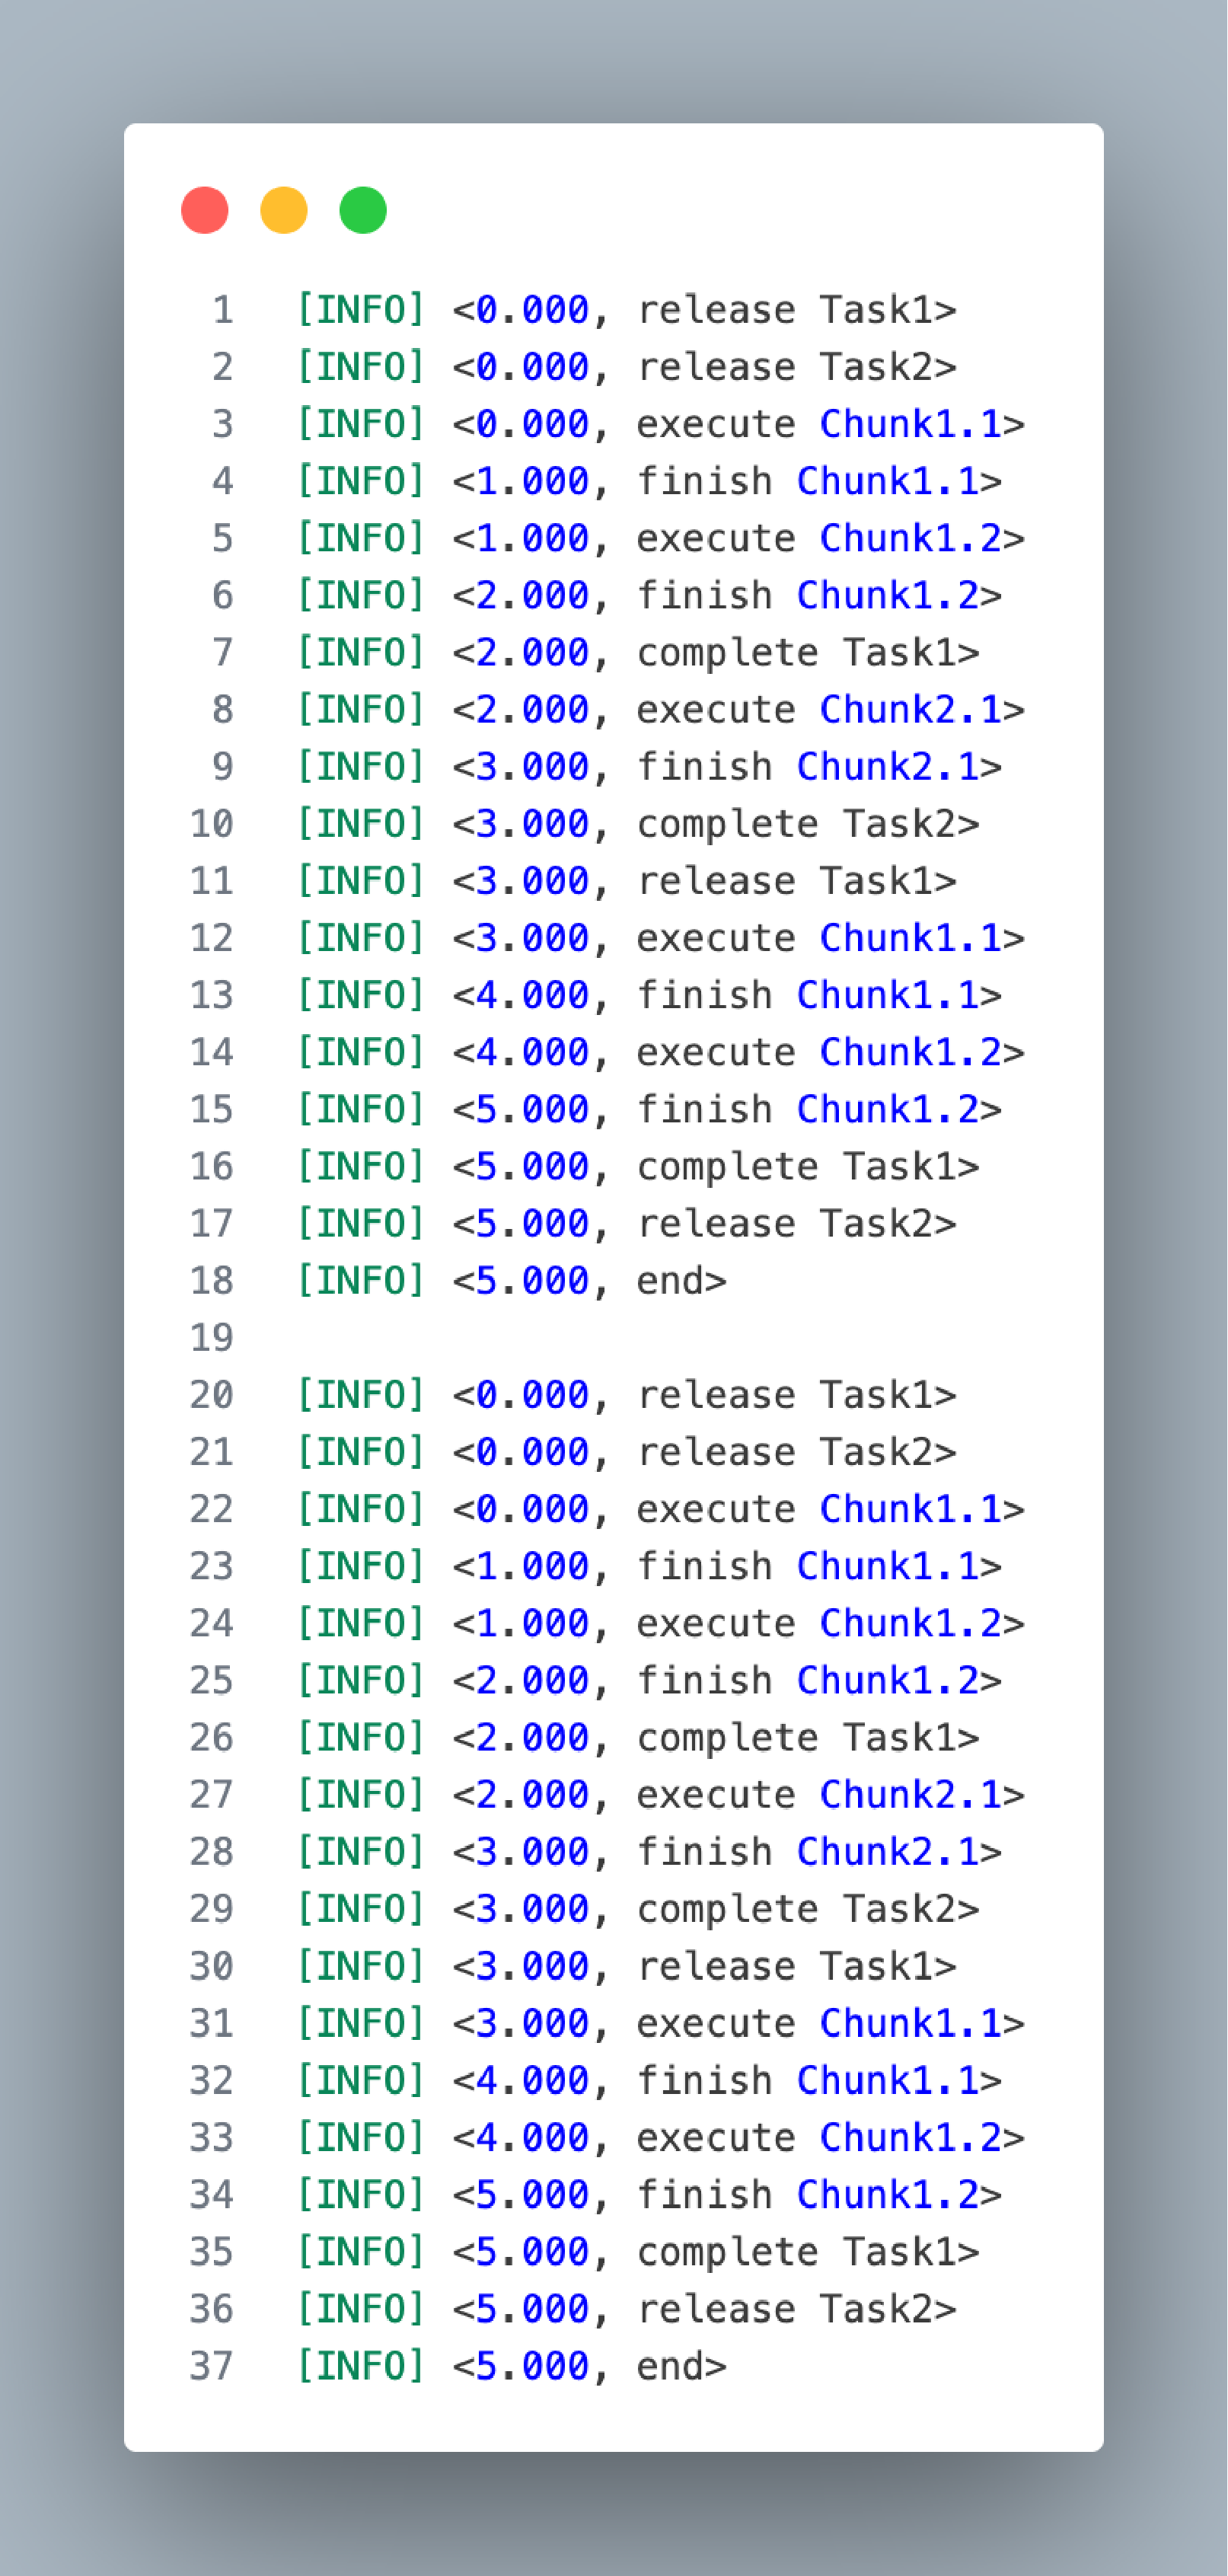
\includegraphics[width=.7\linewidth]{images/2-analisi/trace_management.pdf}
    \caption{\raggedright Trace management example.}
    \label{fig:trace_management}
\end{wrapfigure}

%%%%%%%%%%%%%%%%%%%%%%%%%%%%%%%%%%%%%%%%%
\section{Gestione del tempo}
Un altro aspetto che ha richiesto attenzione è la gestione del tempo.

Siccome Numsynth gestisce valori numerici sia di tipo \textit{int} che \textit{float}~\cite{numsynth}, come prima idea potrebbe venire di utilizzare il tipo \textit{float} e prendere il tempo direttamente dal file di logging. Questo però comporterebbe avere un tempo di training più lungo, vista la complessità nella gestione dei tipi in virgola mobile.

\myskip

Per semplificare l'addestramento è stato quindi deciso di rappresentare il tempo utilizzano \textit{int}.

Siccome il sistema che genera le tracce mostra i tempi in millisecondi con tre cifre decimali, si è moltiplicato per $10^3$ il tempo mostrato. In questo modo è possibile usare tipi interi, ma si deve essere a conoscenza che il tempo va consdierando appunto in microsecondi.

%%%%%%%%%%%%%%%%%%%%%%%%%%%%%%%%%%%%%%%%%
\section{Primo approccio}
Il primo approccio tentato è stato il più semplice possibile: abbiamo inserito come predicati solamente ciò che i log del simulatore di taskset ci forniva. Questi nello specifico sono: rilascio e completmento di un task; inizio e fine dell'esecuzione di un chunk.

In questo modo stiamo chiedendo al sistema di spiegarci il fallimento o il successo della traccia su cui facciamo inferenza solamente tramite questi predicati. Sarà poi Numsynth a cercare di trovare delle relazioni tra chunk e task, anche numeriche, per coprire il maggior numero di esempi positivi e non coprire nessuno di quelli positivi.

A livello implementativo questo si traduce aumentando di un'unità l'arietà di ogni prodicato, in modo da includere la traccia che ha generato quell'evento. Se ad esempio l'aerietà di \textit{release} sarebbe 2, tempo e taskl, questa diventa 3, tempo, task e traccia.